\newpage
\section{Quantity}
\code{Quantity} is used to represent amounts of anything.
Three attributes allow \code{Quantity} to specify everything: a numerical value (\code{BigDecimal}), a (measurement) unit or metric (\code{Metric}), and a type specifying the rounding of the numerical type (\code{RoudingStrategy}), as can be seen in Figure \ref{quantity_overview}.

\code{Quantity} objects are immutable and the class implements the \code{Comparable} interface.

\begin{figure}[ht]
	\centering
  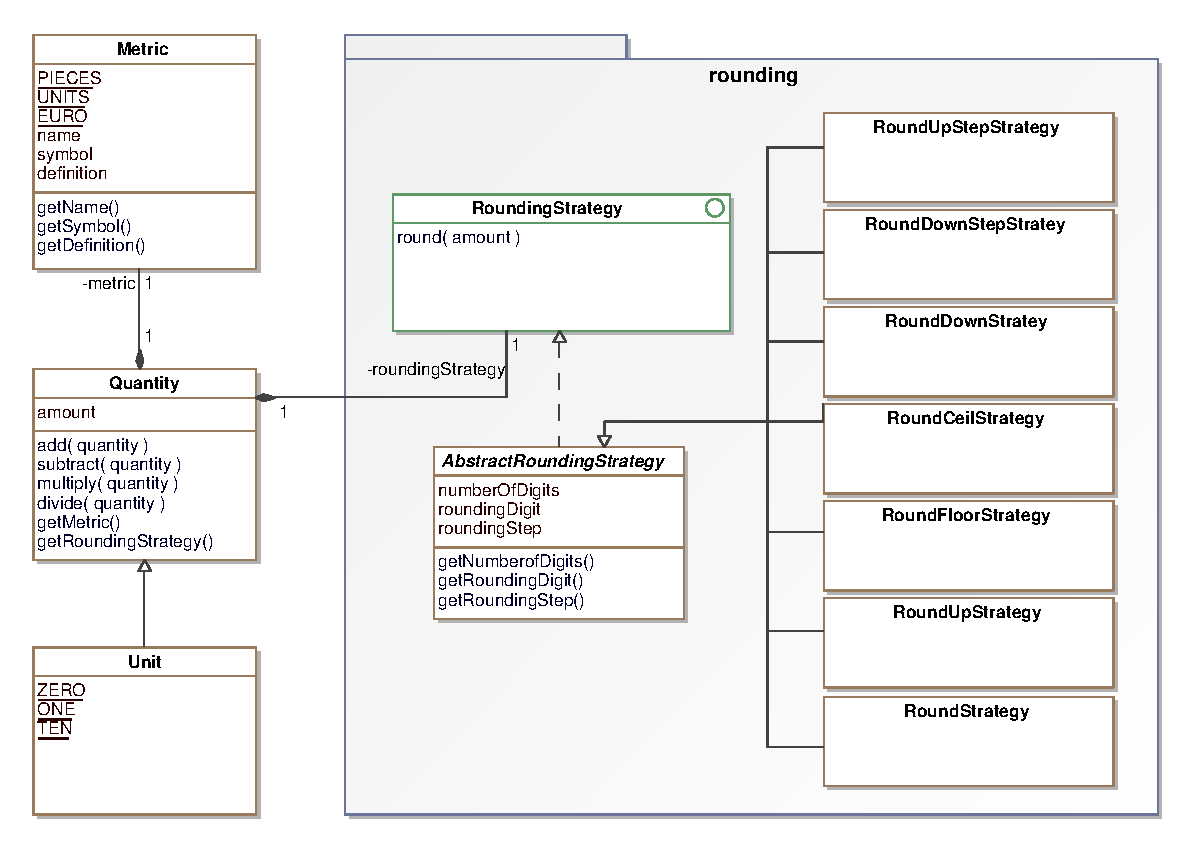
\includegraphics[width=1.0\textwidth]{images/Quantity_Overview.eps}
	\label{quantity_overview}
	\caption{Quantity - Class Overview}
\end{figure}

\subsection{\code{BigDecimal} - Representing numerical values}
\code{BigDecimal} was chosen over \code{float} or \code{double} because of its arbitraty precision.
Moreover, objects of \code{BigDecimal} are immutable and the \code{BigDecimal} class provides operations for including, but not limited to: arithmetic, rounding, and comparison.

\subsection{\code{Metric} - What is represented}
The composite type \code{Metric} contains all information pertaining to the unit or metric of the represented object.
Examples for units or metrics are: m (meter), s (second), pcs (pieces).
Thus, a metric can be described by a symbol (m) and a name (meter).
Furthermore, an object of type \code{Metric} has a description field, to explain the meaning of the metric in detail.

Convenience instances exist for euros, pieces and units.

\subsection{\code{RoundingStrategy} - How to handle half a person}
When handling quantities of unkown metric, standard rounding rules cannot always be employed.
The case of natural persons is just one example, when rounding rules have to be restricted to yield a useful result.
You can round in four general directions: away from zero, towards zero, towards positive infinity, and towards negative infinity.

Additionally, you can specify the digits after the decimal delimiter.
Monetary values in \euro{} or \$US are often just represented with two digits after the decimal delimiter.
Other values, such as kilo grams may be required to be specified to four digits after the decimal delimiter or even further.
In case of (natural) persons, the digits after the decimal delimiter is usually zero, except you are working in statistics (1.45 children per couple) or you are a serial killer dismembering your victims.

The third parameter for rounding is the rounding digit, i.e. the number specifying when you round up or down.
Usually, this number is five.
In case of persons, it is one: if you have $n.0\,persons$, you round down, otherwise up.
If you are calculation a capacity for persons, you will have to round down, this can be done by specifying the correct rouding direction.
\\

Sometimes, it is necessary to round a number to a nearest ``step'', i.e. if you sell something in packs of $50$, and someone punches in $40$, you will have to round up to $50$.
So your rounding step is $50$.
Another example is material, which is sold by the meter or yard.
You have to round the amount specified by your customer accordingly.
Of course, a rouding step can be smaller than $1$, i.e. $0.25$.
\\

Two convenience rounding strategies exist so far: \code{RoudingStrategy.MONETARY} rouding with four digits after the decimal delimiter and rouding towards zero, and \code{RoudingStrategy.ROUND\_ONE} with zero digits after the decimal delimiter and also rouding towards zero.
\\

Rounding is implemented as strategy pattern, but an abstract class (\code{AbstractRoundingStrategy}) is introduced in the pattern (Figure \ref{quantity_overview}).
\code{AbstractRoundingStrategy} contains common methods such as \code{equals()} and \code{hashcode} and getters, thus reducing code repetition.
\subsection{\code{Money} - A usecase for \code{Quantity}}
Objects of class \code{Money} are used to represent amounts of currency within Salespoint.
The following paragraphs detail the intended use, internal modelling and implementation of \code{Money}.
The UML model is given in Figure \ref{money_overview}.

\begin{figure}[ht]
	\centering
  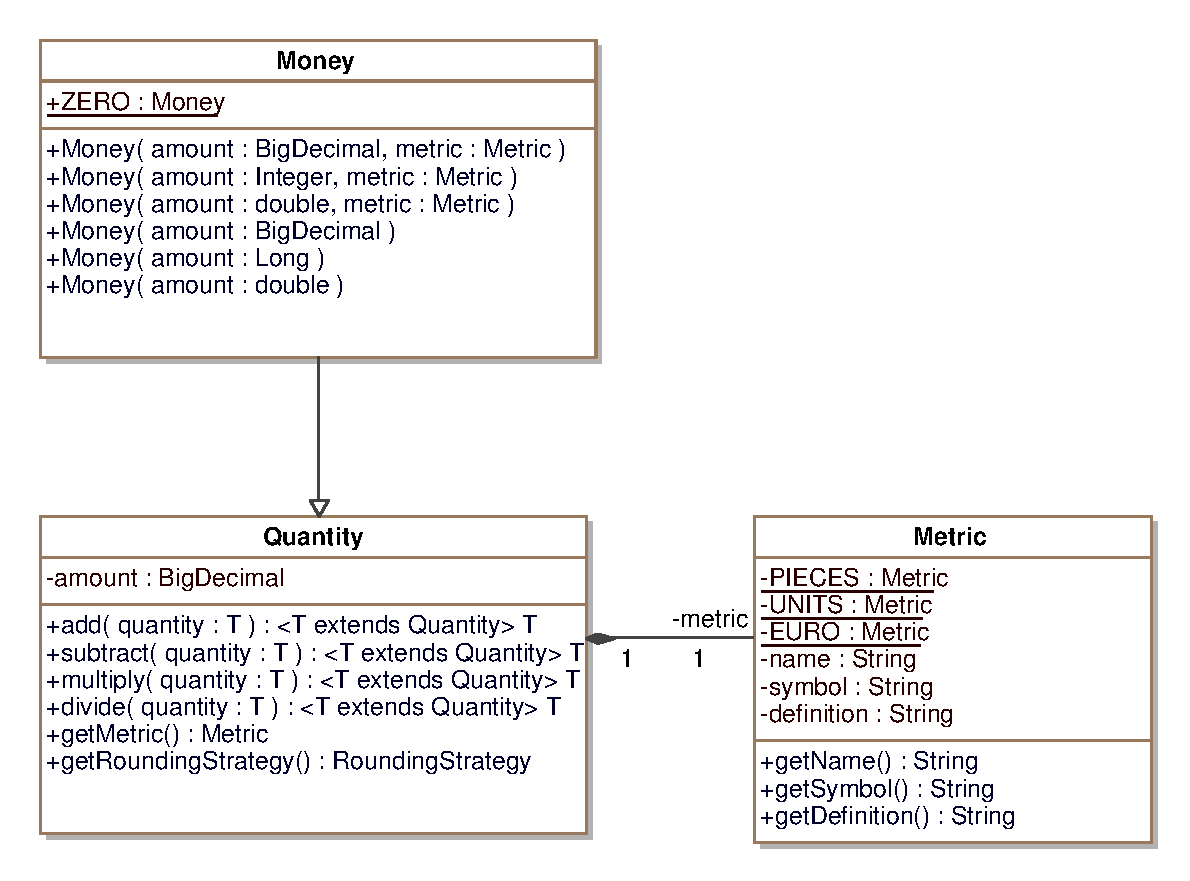
\includegraphics[width=1.0\textwidth]{images/Money_Overview.eps}
	\label{money_overview}
	\caption{Money - Class Overview}
\end{figure}

A \code{Money} object can be instantiated by just passing the numerical value as constructor parameter.
In this case, the metric \code{Metric.EURO} is used, as well as \code{RoundingStrategy.MONETARY} for the rounding strategy attribute.

For other currencies, a \code{Metric} parameter can be passed to the constructor along with a numerical paramter.
However, conversion between currencies is not supported, as it was not deemed necessary.

The rounding strategy cannot be overridden.
Internally, \code{Money} objects calculate with and are rounded to four digits after the decimal delimiter to minimize the rounding error.
The \code{toString()} method, however, limits the output to the expected two digits after the decimal delimiter and appends the symbol of the associated \code{Metric}.

Two convenience instances exist: \code{Money.ZERO}, representing \euro{0,00}, and \code{Money.OVER9000}, representing an amount greater than \euro{9000,00}.

\subsection{\code{Unit} - Representing persons or other integral items}
To represent integral items conveniently, the objects of class \code{Unit} can be used.
The rouding strategy is fixed for all instances to \code{RoundingStrategy.ROUND\_ONE} and \code{Metric.PIECES} is used as metric.
Convenience instances for amounts of zero, one and ten unit(s) exist (\code{Unit.ZERO}, \code{Unit.ONE}, and \code{Unit.TEN}).
